\section{Examples and comparison}
\begin{frame}[fragile]
	\frametitle{Optimization: Interface}
	\begin{columns}
		\begin{column}{0.4\textwidth}
			\begin{itemize}
				\item By balancing the jerk with the velocity we can reduce these overshoots
				      \begin{equation*}
					      \min \int_0^T \alpha \diff{\qv}{t}  + (1-\alpha) \diffk{\qv}{t}{3} \d t
				      \end{equation*}
			\end{itemize}
			\begin{lstlisting}[language=python]

waypoints = np.random.rand(4, 2)

c1 = gsplines.optimization.broken_lines_path(waypoints)
c3 = gsplines.optimization.minimum_jerk_path(waypoints)
c4 = gsplines.optimization.rojas_path(waypoints, 0.8)
c5 = gsplines.optimization.rojas_path(waypoints, 1.5)
c6 = gsplines.optimization.rojas_path(waypoints, 2)

gsplines.plot.plot2d_compare([c1, c3, c4, c5, c6], [
            'green', 'blue', 'magenta', 'red',
            'gray'],
            ['min vel', 'min jerk', 'balance k=0.8',
            'balance k=1.5', 'balance k=2'])
\end{lstlisting}
		\end{column}
		\begin{column}{0.6\textwidth}
			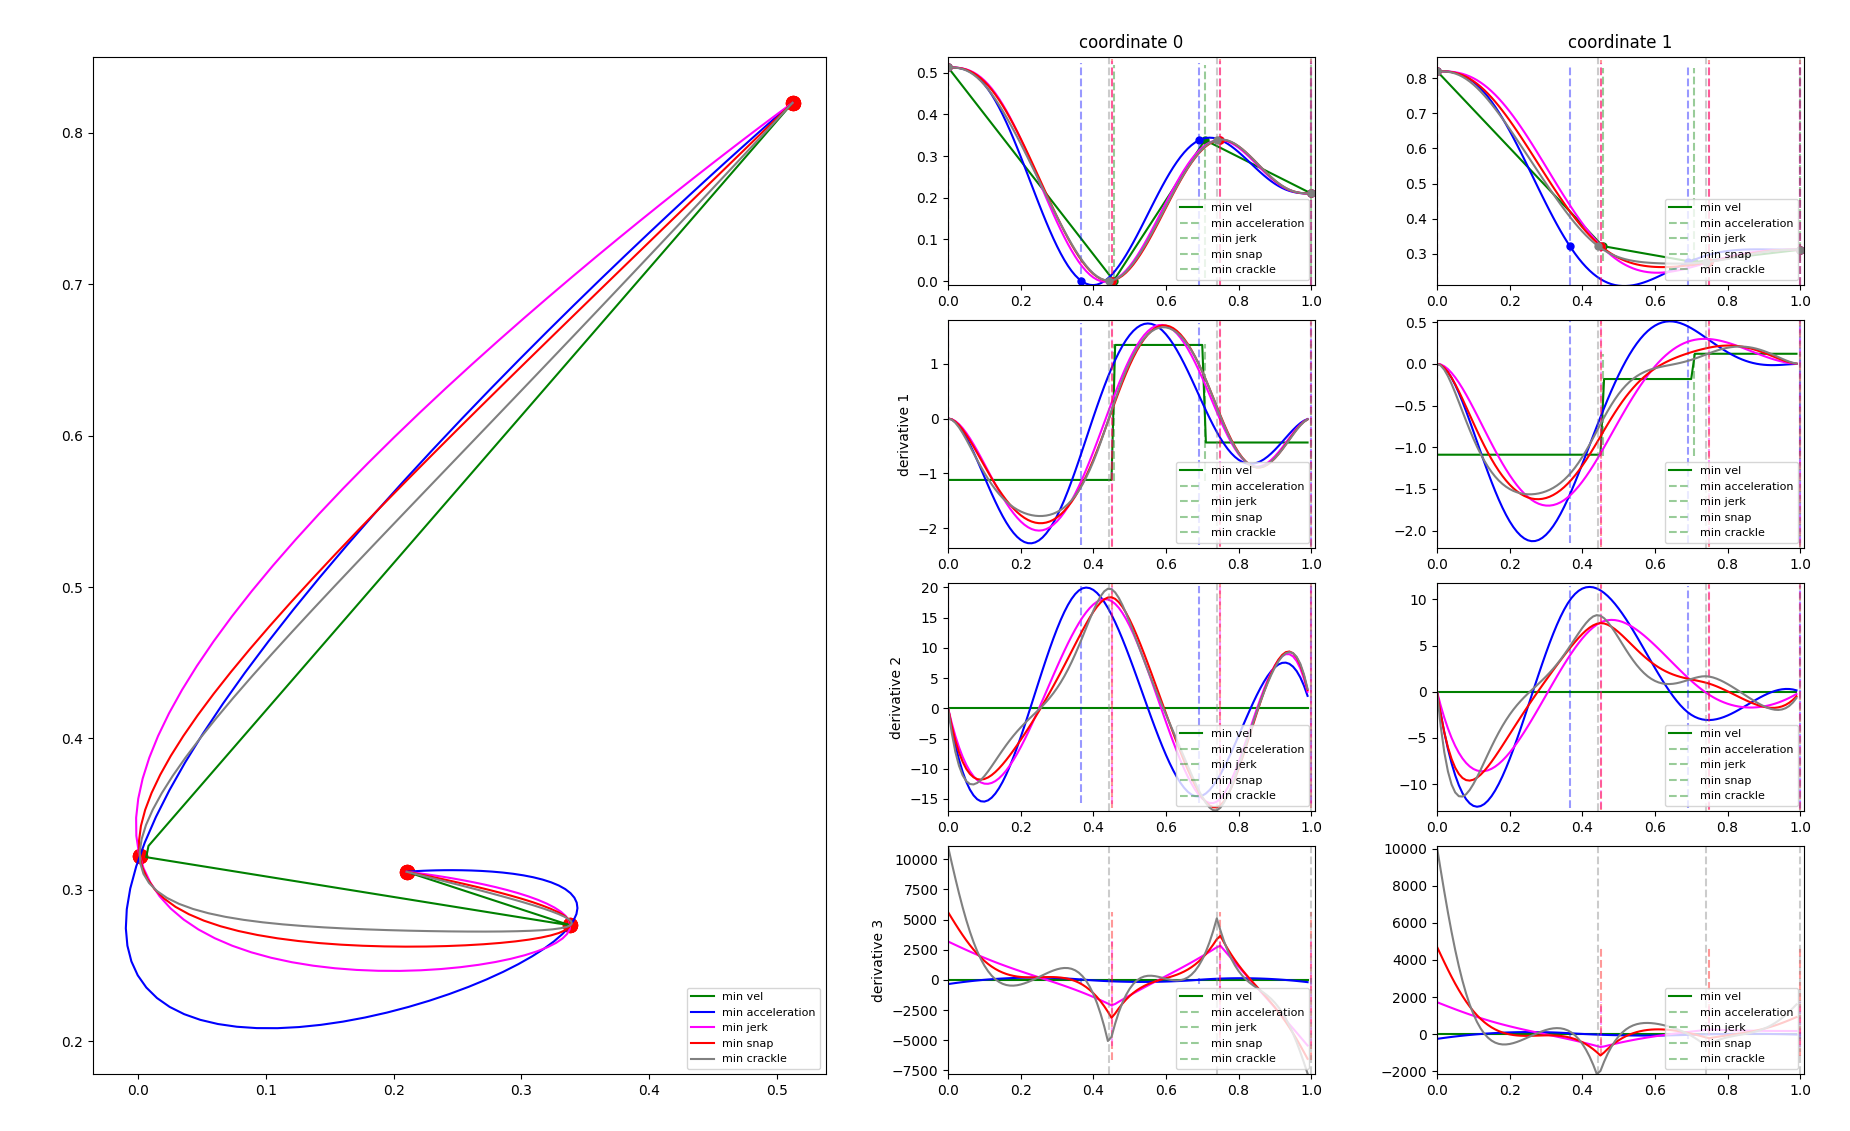
\includegraphics[width=\textwidth]{./images/comparison_2.png}
		\end{column}
	\end{columns}

\end{frame}


\begin{frame}
	\frametitle{A better type of motions}
	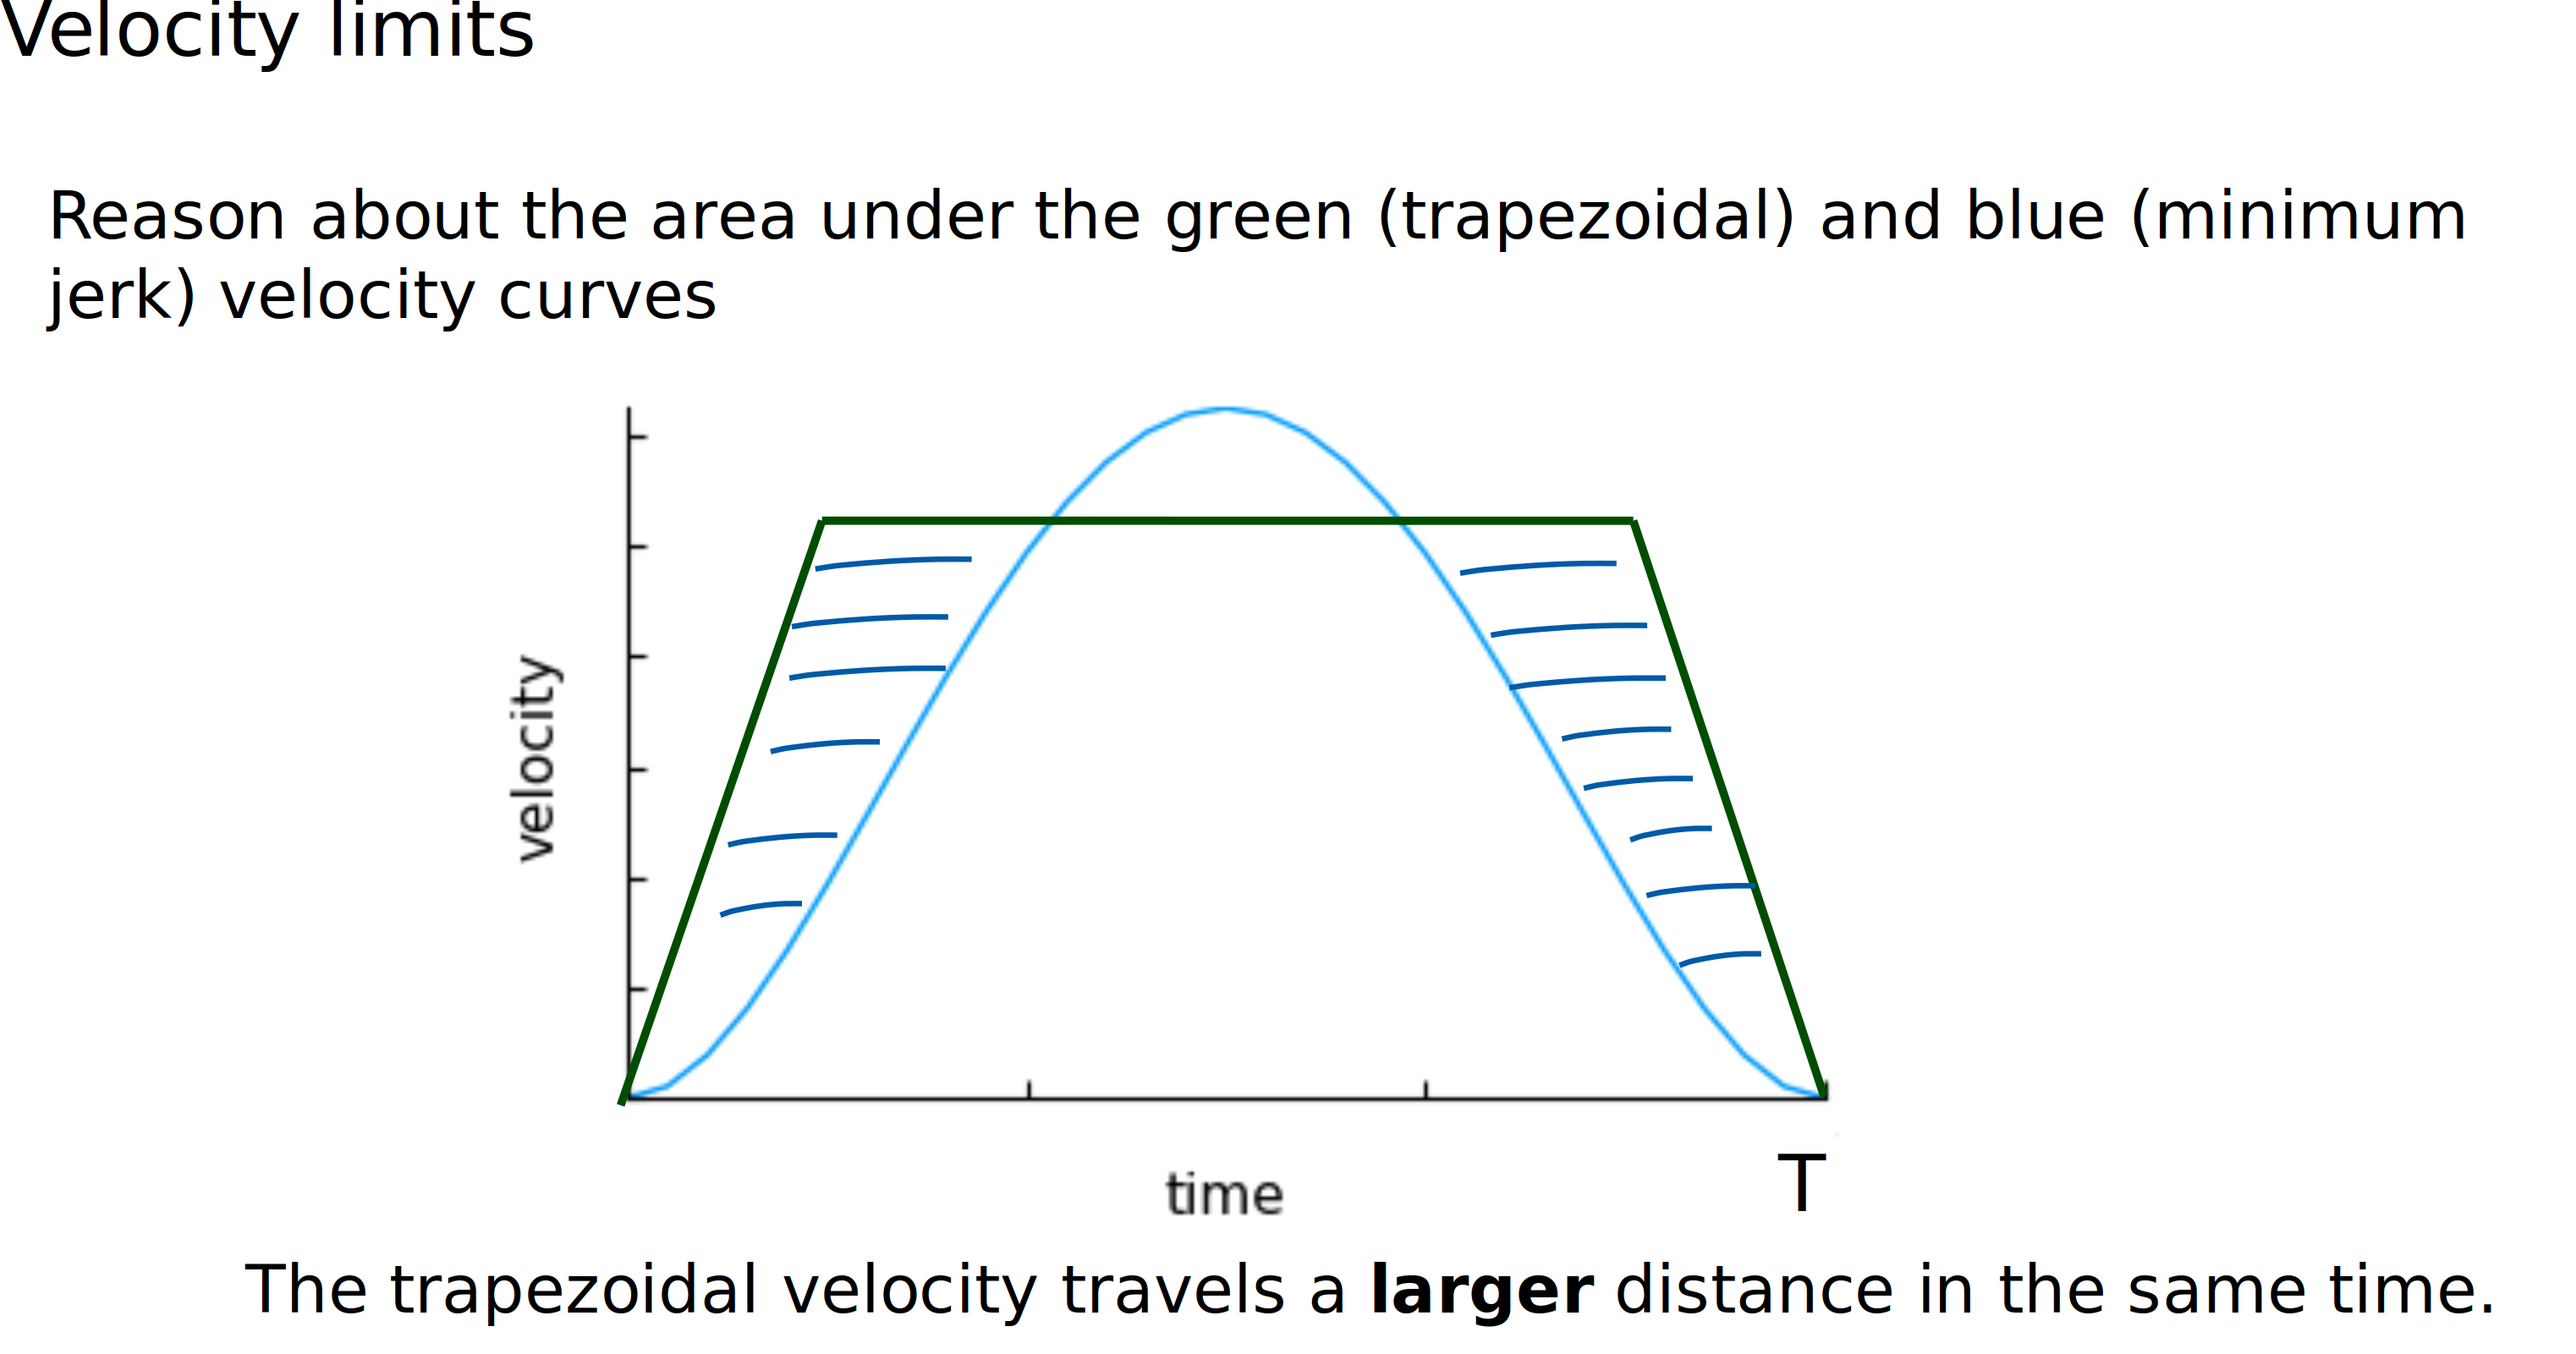
\includegraphics[width=\textwidth]{./images/temporal_slide_trapezoidal_and_corners.png}
\end{frame}

\begin{frame}
	\frametitle{Comparison with Ruckig and Pilz}
\end{frame}

\begin{frame}
	\frametitle{OpStp}
\end{frame}
